\chapter{Preliminaries}\label{preliminaries}
% This \emph{optional} chapter contains the stuff that your reader needs to know
% in order to understand your work.  Your ``audience" consists of fellow third
% year computing science bachelor students who have done the same core courses
% as you have, but not necessarily the same specialization, minor, or free
% electives.
This section will describe malware, the different types and how it utilizes DGA
perform malicious act. It will also explain the basics of Machine Learning and the types of Neural Networks that are necessary for this research paper to comprehend. \\\\ 
Malware is a blending of two words, malicious and
software, where it clearly defines the functionality of it, namely a software
that is malicious in nature. Malware can have multiple purposes. Cybercriminals
typically use it to extract data from the victims computer to leverage against
them for financial gain. This data can range from financial data, sensitive
personal data: such as healthcare records, personal emails, passwords, etc. The
possibilities of the information that can be compromised are endless.\\\\ The
most common ways victims receive malware is through the internet and mail.
Malware can penetrate a victim's computer in different ways, such as: surfing to
hacked websites, viewing malicious ads on websites, download infected files and
install malicious programs or apps. When a malware has infected the computer
system of a victim, it can come in many forms, such as Ransomware, Spyware,
Trojans, Worms, etc.
\section{Botnets}
A compromised machine that is infected
by malware can end up a network of infected machines (botnets). This machine is
a bot in that network that receives and responds to commands from the command \&
control server. The C \& C server is controlled by and receives commands by a
human controller called a botmaster. The botmaster conceals itself by employing
a number of proxy machines, called the stepping stones, between it and the C \&
C server.  
\pagebreak 
The life cycle of a botnet can be divided into four
phases. For this research only the first two phases are important. The first
phase is when the machine (bot) receives the malware and executes the binary.
After the machine is infected, this machine (bot) tries to contact the C \& C
server to announce its presence and contact with it. This establishment phase is
called Rallying. There are two ways that the bot can contact with the C \& C
server. The first way that the bot knows the IP address of the C \& C server.
This IP address can be hardcoded into the binary, which can be exposed 
by reverse engineering the binary. The IP address can also be seeded,
where the bot is provided by a list of peers, this list can be hidden in Windows
registries.  The second way is that the bot knows the domain name of the C \& C
server.  The domain name can be hardcoded into the bot binary, where it can
resolve to different IP addresses.  Reverse engineering this binary may expose
the domain name, which can then be blacklisted.
\section{Domain Generated Algorithm}
The domain name can also be generated, then the bot dynamically contacts the C \& C server using DGA (Domain name Generation Algorithm).  The essence of this algorithm is that it creates a set of random strings. The bot attempts to resolve the generated domain names by sending DNS queries until one of the domains resolves to the C \& C server IP Address. The domains that do not resolve will result in Non-Existent Domain (NXDomain) responses.\\\\ The domain names that are generated by the DGA are also known as Algorithmically Generated Domains (AGD).  The DGA uses a seed to serve as a shared secret between the botmaster and the bot. There are two types of seeds: static seed and dynamic seed. The seed is required to calculate the AGDs. The DGA takes the seed value as input to generate pseudo-random strings and append algorithmically TLD (Top Level domains) such as \textit{.nl, .com, .org, .edu}. The static seed can be dictionary of words, random strings that are concatenated, numbers or any other value that the botmaster can come up with. Dynamic seeds are dynamic, it changes with time. Dynamic seeds can be currency exchange rate, daily trending twitter hashtag, weather temperature and current date and time.  The static and dynamic seed elements are then stitched together to generate a pseudo-random string.\\\\ The botmaster uses the DGA to generate a large number of domain names for the C \& C server.  The constant change of domain names for the C \& C server using DGA is known as Domain-Fluxing.  The botmaster registers one of the DGA created domain names for the C \& C server in advance using the same algorithm of the DGA.  When the bot receives the malware, the malware queries to the pre-registered domain name and resolves the IP address using DNS.  The botmaster registers the domain name most of the time some hours prior to an attack and disposes of the domain names within a day.  Whenever the previous domain name that the bot connected with does not resolve anymore, it queries to the next set of generated domain names until it find one domain that works.\\\\ The DGA and constant domain-fluxing of the C \& C server provides agility and resilience to the infrastructure of the botmaster.  This makes it hard to predict what domain names a bot will try. Analyst will re-engineer DGA by analyzing the malware and understand how the algorithm works. It is still hard to predict what kind of seed the DGA will use on a specific time. It is also infeasible to report all the domain names that are generated. As some DGA use english dictionary as static seed values, it is hard to distinguish benign domain names from malicious ones.  
\section{Machine Learning}
Machine learning has recently been an attractive tool to be used in security. One way to combat DGA is to use machine learning to find the structure of the generated domains. The machine learning methods can be either supervised or unsupervised. Unsupervised learning uses algorithms to analyze and cluster data, in this case the domains. These algorithms discover hidden patterns or data groupings, without a need for a human intervention. There are three ways to approach unsupervised learning: clustering, association and dimensionality reduction. The domains are divided into clusters to find statistical attributes for each group. To produce a cluster with good generalization capabilities, it can take a lot of time and  effort \cite{unsupervised}. Supervised learning does not rely on the statistical attributes  for each group to find DGAs. Supervised learning attempts to understand and classify the input and predict the outcome accurately. The relationship is represented as a structure to predict the outputs for some specific future inputs.  
\subsection{Neural Networks}
Artificial Neural Networks are artificial systems that were inspired by the biological counterpart. The systems learn in a supervised manner to perform tasks by using various datasets and examples. These neural networks are composed of node layers, containing one or more input layers, hidden layers and output layers. Each node is connected to another node and has an associated weight w and threshold. When the threshold of a specific node is above a certain threshold value, then that node is activated, otherwise no data is passed along to the next layer of the network. \\\\ 
The network uses training data to learn and improve the accuracy of the network. This is usually done by backpropagation. Backpropagation is a supervised learning algorithm that computes the difference between the model output and the actual output using gradient descent\cite{gradient_descent}. It checks if the error is minimized and update the weights and biases accordingly. It repeats the process until the error becomes minimum.  

\subsection{Activation Functions}
The activation functions in a neural network are functions that determine the output of a neural network. It maps it to a specific value. The function receives the calculated weighted sum of the inputs and the added bias and then decides if this passes through or not. \\\\
There are two types of activation functions: Linear Activation function and Non-linear Activation Functions.
The linear activation functions are functions that does not change the weighted sum of the input, but instead returns the value directly. For multiple layer networks we need non-linear activation function.

\subsubsection{ReLU}
ReLU, or Rectified Linear Unit, is linear when the input is positive and 0 when the input is negative. The range of ReLu is [0, inf). The benefit of ReLu is that there is a reduced likelihood of the gradient to vanish(see subsection Vanish Gradient Problem), as the gradient is constant. THis constant gradient results in faster learning of the network. Another benefit is the sparsity, as the network has more units in a layer, other activation functions will be processed to describe the output of that network. When the calculated sum that goes into the activation of ReLu is negative, it yields 0. This means there is fewer neurons firing, which makes the network lighter.\\\\
The disadvantage is that it tends to blow up, as the range goes to infinity and there is no mechanism to constrain the output when it is positive. Another disadvantage is the problem that if too many activations in the network get below zero, than the neurons in the network will output zero. This means that the outputs die out, thus prohibiting learning. This is called the Dying ReLu problem.

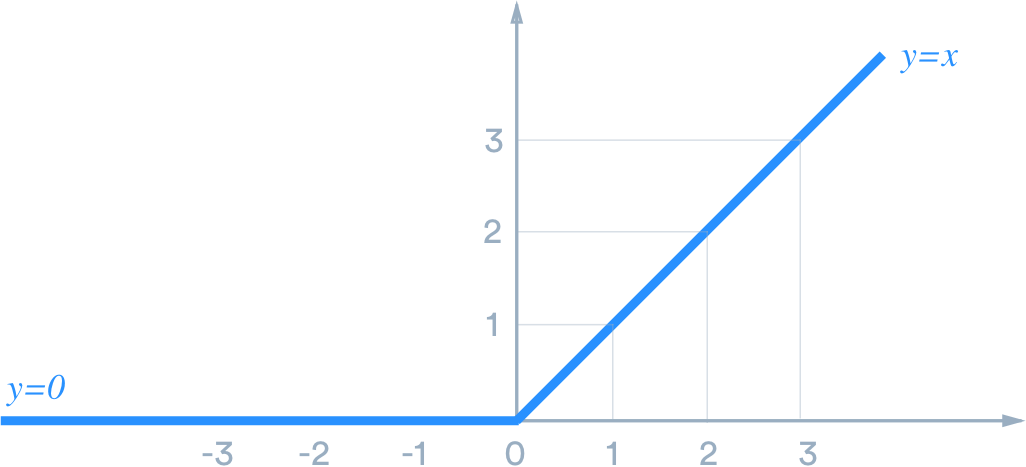
\includegraphics{relu}


\subsubsection{Sigmoid}
Sigmoid activation function is a non-linear activation function that looks like an S-shape. Any small changes in the incoming X value(the calculated sum) will cause the Y value (the output) to change significantly. The range is [0,1], so it is bounded in a range and it does not blow up. The disadvantage of the Sigmoid function is the vanishing gradients(see subsection Vanishing Gradient Problem)

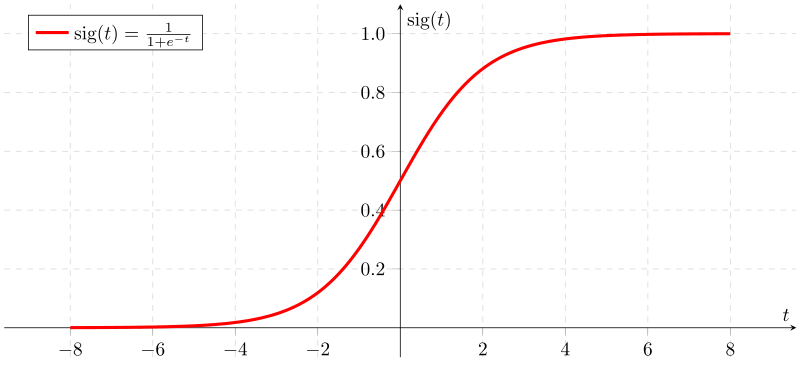
\includegraphics{sigmoid_function}

\subsubsection{Tanh}
The Tanh activation function is very similar to the Sigmoid function. The difference is that the range is ]-1,1] and the gradient is stronger for tanh than sigmoid. That means the derivative are steeper. One benefit of tanh over sigmoid is that it avoids bias in the gradients \cite{tanh}.

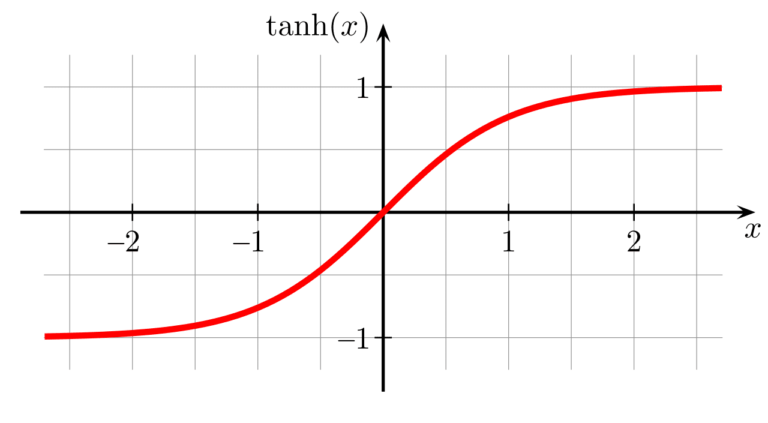
\includegraphics{tanh_function}

\subsection{Recurrent Neural Networks}
Recurrent neural networks are a type of neural network that uses the output from the previous step and fed that as input in the current step, while in traditional Neural networks the network assumes that the inputs and outputs are independent of each other. It is known for its feedback loops. Recurrent Neural Networks are used for Sequence Modeling. Sequence Modeling is the task to predict about future outcomes. 


\subsection{Vanishing Gradient problem}
\subsection{LTSM}
\subsection{The core of LTSM}
\subsection{Transformers}